% Experiments. All numbers come from numbers.tex / numbers_results.tex and tables/*.tex.

\section{Experiments}
\label{sec:experiments}

\subsection{Setup}
\label{sec:setup}

\paragraph{Datasets and metrics.}
We use UCF-Crime~\cite{sultani2018real} and XD-Violence~\cite{wu2020xdviolence} with the CLIP snippet features, splits, and frame-level ground truth released with VadCLIP~\cite{wu2024vadclip}. The test sets contain 290 and 800 videos. Following VadCLIP, the headline metric is frame-level AUC of $s^{(1)}$ on UCF-Crime and frame-level AP of $p$ on XD-Violence. Because the two datasets are headlined on different outputs, we also report the other output on each dataset.

\paragraph{Training protocol.}
The released VadCLIP training script evaluates the model on the test set after every epoch, keeps the checkpoint with the best test AP, and reloads it before the next epoch. We train every model for a fixed 10 epochs and evaluate the final checkpoint, so training and checkpoint selection use training data only. All other settings follow the released configuration of each dataset. Each condition is trained with seeds 234, 235, and 236. Runs that share a seed share initialization and sample order, and we report paired differences per seed together with the number of seeds on which the difference is positive.

With our evaluator, VadCLIP's released checkpoints reach \ucfOfficial{} AUC on UCF-Crime and \xdOfficial{} AP on XD-Violence. The XD-Violence value is within \xdReadmeGap{} points of the \xdReadmeAp{} reported in the VadCLIP repository. VadCLIP retrained under our protocol reaches \ucfRetrained{} AUC and \xdBase{} AP, and all comparisons below use this retrained baseline unless stated otherwise. Section~\ref{sec:official} repeats the main XD-Violence comparison under VadCLIP's official training script.

\subsection{Comparison with published methods}
\label{sec:sota}

% Auto-generated by scripts/make_tables.py. Do not edit by hand.
\begin{table}[t]
\centering
\small
\setlength{\tabcolsep}{4pt}
\caption{Published results with CLIP features (\%), as reported in VadCLIP~\cite{wu2024vadclip}; these use each method's own training and model-selection protocol. Rows below the first rule are our three-seed means under the test-independent protocol; rows below the second rule use VadCLIP's official script, which selects checkpoints on the test set. Only rows within a block are directly comparable.}
\label{tab:sota}
\begin{tabular}{lcc}
\toprule
Method & UCF AUC$_1$ & XD AP$_2$ \\
\midrule
Sultani et al.~\cite{sultani2018real} & 84.14 & 75.18 \\
Wu et al. (HL-Net)~\cite{wu2020xdviolence} & 84.57 & 80.00 \\
RTFM~\cite{tian2021rtfm} & 85.66 & 78.27 \\
UR-DMU~\cite{zhou2023urdmu} & 86.75 & 82.41 \\
CLIP-TSA~\cite{joo2023cliptsa} & 87.58 & 82.17 \\
VadCLIP~\cite{wu2024vadclip} & 88.02 & 84.51 \\
\midrule
VadCLIP, retrained (ours) & 86.25$\pm$0.83 & 77.57$\pm$2.19 \\
Ours & 86.53$\pm$0.85 & 79.23$\pm$1.87 \\
\midrule
VadCLIP, official script (ours) & -- & 82.91$\pm$1.23 \\
Ours, official script & -- & 83.63$\pm$1.18 \\
\bottomrule
\end{tabular}
\end{table}


Table~\ref{tab:sota} lists published results with CLIP features as reported in VadCLIP~\cite{wu2024vadclip}, together with our three-seed means. Published numbers come from each method's own training and model-selection protocol, and VadCLIP's are obtained with a script that selects checkpoints on the test set. Under our test-independent protocol, retrained VadCLIP reaches \ucfRetrained{} AUC and \xdBase{} AP, below its reported values, so absolute numbers in the first block are not comparable with ours. Within each of the other two blocks, both arms share the protocol and seeds, and our method is higher than VadCLIP in both.

\subsection{Controlled comparison}
\label{sec:controlled}

% Auto-generated by scripts/make_tables.py. Do not edit by hand.
\begin{table}[t]
\centering
\small
\setlength{\tabcolsep}{4pt}
\caption{Controlled comparison under the test-independent protocol (mean$\pm$SD over seeds 234--236, \%). Paired $\Delta$ is computed per seed; parentheses give the number of positive seeds. Headline metrics follow VadCLIP: AUC of $s^{(1)}$ on UCF-Crime and AP of $p$ on XD-Violence.}
\label{tab:controlled}
\begin{tabular}{lcccc}
\toprule
Method & UCF AUC$_1$ & UCF AP$_2$ & XD AP$_2$ & XD AP$_1$ \\
\midrule
VadCLIP, retrained & 86.25$\pm$0.83 & 26.46$\pm$1.20 & 77.57$\pm$2.19 & 79.61$\pm$0.86 \\
Ours & 86.53$\pm$0.85 & 27.30$\pm$1.60 & 79.23$\pm$1.87 & 79.54$\pm$0.97 \\
Paired $\Delta$ & +0.28$\pm$0.15 (3/3) & +0.85$\pm$0.42 (3/3) & +1.66$\pm$0.34 (3/3) & $-$0.06$\pm$0.11 (1/3) \\
\bottomrule
\end{tabular}
\end{table}


\begin{figure}[t]
  \centering
  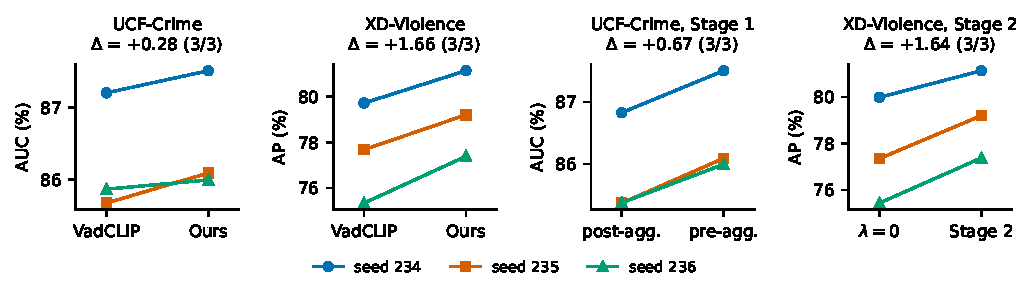
\includegraphics[width=\linewidth]{figures/fig_paired.pdf}
  \caption{Paired per-seed results under the test-independent protocol. Each line connects the two arms of one seed; the title gives the mean paired difference in points and the number of positive seeds. Left to right: full method against retrained VadCLIP on UCF-Crime (AUC) and XD-Violence (AP), pre- against post-aggregation variation in Stage~1, and Stage~2 against the equal-budget control with $\lambda = 0$.}
  \label{fig:paired}
\end{figure}

Table~\ref{tab:controlled} compares our method with VadCLIP retrained under the same protocol and seeds. On UCF-Crime, AUC improves by \ucfGainMean{} points ($\pm$\ucfGainSd, \ucfGainPos{} seeds). On XD-Violence, AP improves by \xdGainMean{} points ($\pm$\xdGainSd, \xdGainPos{} seeds). Both arms of each pair share initialization and sample order, so the paired difference removes variation common to a seed, and it is positive on every seed for both datasets (Fig.~\ref{fig:paired}). The XD-Violence gain is on the semantic output that VadCLIP uses for its XD-Violence headline, and AP of $s^{(1)}$ changes by \xdApOneChangeMean{} points.

\subsection{Results under the official training protocol}
\label{sec:official}

% Auto-generated by scripts/make_tables.py. Do not edit by hand.
\begin{table}[t]
\centering
\small
\setlength{\tabcolsep}{4pt}
\caption{XD-Violence AP$_2$ (\%) under VadCLIP's official training script, which evaluates on the test set after every epoch and keeps and reloads the best checkpoint. B0 and Ours are trained with the same script and seed. $\Delta$ is the paired difference; parentheses give the number of positive seeds.}
\label{tab:official}
\begin{tabular}{lccc}
\toprule
Seed & VadCLIP (B0) & Ours & $\Delta$ \\
\midrule
234 & 84.21 & 84.94 & +0.73 \\
235 & 81.77 & 82.65 & +0.88 \\
236 & 82.74 & 83.31 & +0.57 \\
\midrule
Mean & 82.91$\pm$1.23 & 83.63$\pm$1.18 & +0.73$\pm$0.16 (3/3) \\
\bottomrule
\end{tabular}
\end{table}


To check that the gain is not specific to our training protocol, we also train VadCLIP and our method on XD-Violence with VadCLIP's official training script, which evaluates on the test set after every epoch and keeps and reloads the best checkpoint. Both arms use the script unchanged and the same seeds 234, 235, and 236; these runs were made on an RTX 4090. Under this protocol our method improves AP from \offBase{} to \offOurs{}, a paired gain of \offGainMean{} points ($\pm$\offGainSd, \offGainPos{} seeds; Table~\ref{tab:official}). The gain is positive on every seed under both protocols. Absolute AP is higher for both arms under the official script, so we compare methods only within a protocol. The ablations below use the test-independent protocol.

\subsection{Stage 1: where variation is computed}
\label{sec:ablation}

% Auto-generated by scripts/make_tables.py. Do not edit by hand.
\begin{table}[t]
\centering
\small
\setlength{\tabcolsep}{4pt}
\caption{Placement of temporal variation in Stage 1 (test-independent protocol, \%). Pre-aggregation computes variation on raw snippets; post-aggregation computes it on the pooled sequence with all other settings fixed. $\Delta$ is the paired difference to B0.}
\label{tab:stage1}
\begin{tabular}{lcccc}
\toprule
Variant & UCF AUC$_1$ & $\Delta$ & XD AP$_2$ & $\Delta$ \\
\midrule
VadCLIP (B0) & 86.25$\pm$0.83 & -- & 77.57$\pm$2.19 & -- \\
Stage 1, pre-aggregation (Ours) & 86.53$\pm$0.85 & +0.28$\pm$0.15 (3/3) & 77.44$\pm$2.52 & $-$0.14$\pm$0.33 (1/3) \\
Stage 1, post-aggregation & 85.86$\pm$0.84 & $-$0.39$\pm$0.10 (0/3) & -- & -- \\
\bottomrule
\end{tabular}
\end{table}


Stage~1 produces the UCF-Crime gain, since Stage~2 leaves $s^{(1)}$ unchanged by construction. Table~\ref{tab:stage1} isolates the placement of the difference. We train Stage~1 with variation computed after aggregation, $D'_j = \lvert A_j - A_{j-1} \rvert$, and keep every other setting fixed. This variant falls below the baseline by \postBaseMean{} points on every seed, whereas computing variation before aggregation is better than after it by \prePostMean{} AUC points ($\pm$\prePostSd, \prePostPos{} seeds). The position of the difference relative to pooling therefore determines the gain. The two variants receive identical inputs on videos shorter than $T$, which are only padded, and differ on the long training videos that are averaged (Sec.~\ref{sec:pvr}) and at test-window boundaries.

On XD-Violence, Stage~1 alone changes AP by \xdStageOneMean{} points (\xdStageOnePos{} seeds).
\subsection{Stage 2: semantic post-training}
\label{sec:stage2}

% Auto-generated by scripts/make_tables.py. Do not edit by hand.
\begin{table}[t]
\centering
\small
\setlength{\tabcolsep}{4pt}
\caption{Stage 2 on XD-Violence (test-independent protocol, \%). C and Stage 2 start from the same Stage 1 checkpoint and sample order and differ only in $\lambda$. AP$_1$ is unchanged by Stage 2 by construction.}
\label{tab:stage2}
\begin{tabular}{lccc}
\toprule
Variant & XD AP$_2$ & $\Delta$ vs.\ B0 & XD AP$_1$ \\
\midrule
VadCLIP (B0) & 77.57$\pm$2.19 & -- & 79.61$\pm$0.86 \\
Stage 1 & 77.44$\pm$2.52 & $-$0.14$\pm$0.33 (1/3) & 79.54$\pm$0.97 \\
Stage 1 + CLASM only (C) & 77.59$\pm$2.28 & +0.02$\pm$0.30 (2/3) & 79.54$\pm$0.97 \\
Stage 1 + Stage 2 (Ours) & 79.23$\pm$1.87 & +1.66$\pm$0.34 (3/3) & 79.54$\pm$0.97 \\
B0 + Stage 2 & 79.46$\pm$1.48 & +1.89$\pm$0.76 (3/3) & 79.61$\pm$0.86 \\
\bottomrule
\end{tabular}
\end{table}


An equal-budget control isolates the semantic objective. The control C runs the same three epochs from the same checkpoint and sample order with $\lambda = 0$, and the semantic objective adds \tMinusCMean{} AP points over it ($\pm$\tMinusCSd, \tMinusCPos{} seeds). Applied directly to the retrained VadCLIP, Stage~2 improves AP by \bzTMean{} points ($\pm$\bzTSd, \bzTPos{} seeds), so the XD-Violence gain of the full method is attributable to Stage~2. Placing Stage~1 before it changes AP by a further \tMinusBzTMean{} points (\tMinusBzTPos{} seeds). On UCF-Crime, Stage~2 changes AP of $p$ by \ucfApTwoStageTwoMean{} points.

Throughout Stage~2 training, the maximum change of $s^{(1)}$ on a fixed probe batch was zero and no parameter outside $\mathrm{mlp}_1$ changed.

\subsection{Complexity}
\label{sec:complexity}

% Auto-generated by scripts/make_tables.py. Do not edit by hand.
\begin{table}[t]
\centering
\small
\setlength{\tabcolsep}{4pt}
\caption{Inference cost per window of 256 snippets (batch 1, median of 200 passes after 20 warm-up passes, including prompt encoding). Parameters exclude the frozen CLIP encoders.}
\label{tab:complexity}
\begin{tabular}{llrrr}
\toprule
Data & Model & Params & Latency (ms) & Peak mem.\ (MB) \\
\midrule
UCF & VadCLIP & 12{,}642{,}306 & 28.9 & 670 \\
 & Ours & 12{,}775{,}042 & 29.8 & 671 \\
XD & VadCLIP & 9{,}489{,}922 & 17.4 & 643 \\
 & Ours & 9{,}622{,}658 & 18.1 & 644 \\
\bottomrule
\end{tabular}
\end{table}


Stage~1 adds \pvrParams{} parameters and Stage~2 adds none. On an \cxGpu{}, inference latency rises by \cxUcfLatRel\% on UCF-Crime and \cxXdLatRel\% on XD-Violence, and peak memory by at most \cxUcfMemDelta{} MB (Table~\ref{tab:complexity}).
